\newpage
\section{Inverting a card}
\genHeader
\hypertarget{sec:invertCard}{}

This next SDM \emph{inverts} a card by swapping its back and face values (Fig.~\ref{fig:goal_invert}). This therefore ``turns a card around'' in the learning
box. This action makes sense if a user wants to try learning, for example, the definition of a word in the opposite direction. Instead of guessing the
definition of every word when presented with the term, perhaps they would like to guess the term when presented with the defintion. This method doesn't need to
accept any paramters, as it uses a bounded \texttt{this} variable.

\vspace{0.5cm}

\begin{figure}[htbp]
	\centering
    \includegraphics[width=0.4\textwidth]{invert.pdf}
 	\caption{Inverting the attributes of a \texttt{Card}}
 	\label{fig:goal_invert}
\end{figure}
\FloatBarrier

\vspace{0.5cm}
\begin{itemize}
\item[$\blacktriangleright$] Click on a link below to begin.
\end{itemize}

\begin{center}{$\triangleright$ \hyperlink{invertCard vis}{Inverting a Card: The visual syntax}}%
\\ \vspace{0.5cm}
{$\triangleright$ \hyperlink{invertCard tex}{Inverting a Card: The textual syntax}} \end{center} 



\newpage
\subsection{Implementing invert}
\visHeader
\hypertarget{invertCard vis}{}

\begin{itemize}

% Make sure you explain how/why the green box. Hasn't been convered yet
\item[$\blacktriangleright$] Model the SDM depicted in Fig.~\ref{fig:sdm_invert}. Remember, the green creational object variable is made by setting the binding
operator as \texttt{create}.

% Explain how to use the new assignments??

\vspace{1cm}

\begin{figure}[htbp]
\begin{center}
  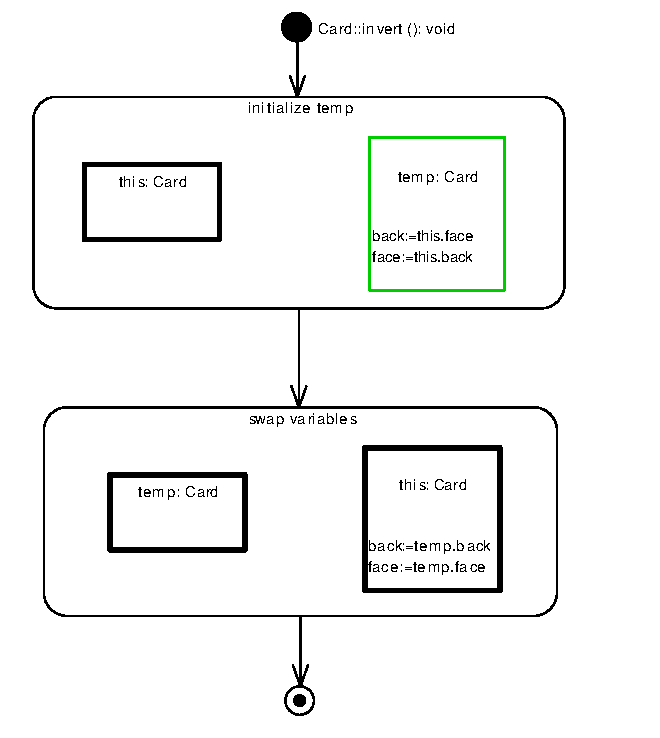
\includegraphics[width=0.9\textwidth]{ea_swappingCard.pdf}
  \caption{Swap back and face of the card}  
  \label{fig:sdm_invert}
\end{center}
\end{figure}

\item[$\blacktriangleright$] Believe or not, that's it! Check out how this method was implemented in the textual syntax by reviewing
Fig.~\ref{fig:invertPatterns} in the next section.

\end{itemize}


\newpage
\subsection{Textual; Turning Cards}
\texHeader
\hypertarget{invertCard tex}{}

\begin{itemize}

\item[$\blacktriangleright$] You're no longer an SDM beginner, so create two patterns in the invert declaration, named \texttt{initializeTemp} and
\texttt{swapVariable}. The only flow this method requires is that these pattern are performed in order - there's no assertion, and it only needs to be
performed once. Don't forget to include a return statement!

\item[$\blacktriangleright$] Your declaration should now resemble Fig.~\ref{fig:eclipse_invert}

\begin{figure}[htbp]
\begin{center}
  \includegraphics[width=0.4\textwidth]{eclipse_invertControlFlow}
  \caption{Control flow for \texttt{card.invert}}  
  \label{fig:eclipse_invert}
\end{center}
\end{figure}

\item[$\blacktriangleright$] Create two bounded object variables in each pattern, and complete the rules until your patterns resemble
Fig.~\ref{fig:invertPatterns}.

\begin{figure}[htbp]
\begin{center}
  \includegraphics[width=0.5\textwidth]{eclipse_invertPatterns}
  \caption{Swap Patterns}  
  \label{fig:invertPatterns}
\end{center}
\end{figure}

\item[$\blacktriangleright$] Believe it or not, that's it! We reccommend building at this point, just to confirm nothing has gone wrong with your metamodel. To
see this method in the visual syntax, review Fig.~\ref{fig:sdm_invert}.

\end{itemize}